\newpage

\section{Trigger}
\label{sec:trigger}

%{\bf data plots needs to be updated for HZ selections}
We use the same triggers as in Section~\ref{sec:trigger1}. 
Events are selected if one of the following triggers has fired:
HLT\_HT750, HLT\_PFHT650, HLT\_PFNoPUHT650, \\
HLT\_FatDiPFJetMass750\_DR1p1\_Deta1p5. Figures~\ref{fig:trigger efficiencies part1}, \ref{fig:trigger efficiencies part2} 
and \ref{fig:trigger efficiencies part3} show the trigger efficiency.
%trigger efficiencies of the OR of the highest threshold HLT\_PFHT650
%trigger efficiencies of the OR of the lowest unprescaled HLT\_PFHT650
%trigger and the HLT\_FatJetMass trigger.  
The trigger efficiency has been
measured with respect to a lower-thrseshold, but prescaled, HLT\_HT550 trigger.  
The trigger is $99\%$ effiecient above 890\GeVcc for the untagged, 
HbbVqq-tagged , and HwwVqq-tagged data.

Figure~\ref{fig:referencetrigger} shows the turn-on curve of the reference trigger on 
the signal MC. The 1.0\TeVcc signals are used here in Figure~\ref{fig:referencetrigger}, and
the plot shows that the HwwVqq and HbbVqq signals are  
fully efficient for HLT\_HT550 trigger, which is not prescaled in MC. So other signals,
having resonance mass bigger than 1.0 \TeVcc, will surely be fully efficient for the triggers. 

%The turn on curve of the reference trigger, HLT\_HT550 is checked in our signal MC, 
%which is fully efficient above 890 \GeV, as shown in Figure.~\ref{fig:referencetrigger}. 
%For signal with resonances above 1.0 \TeV, the reference trigger is fully efficient 
%above 890 \GeV for sure. 

%This trigger study checks for a WW final state rather than a WH final state. 
%Our H tagger use a heavier mass window than W-tagger,
% which will result in higher resonance 
%mass in WH final state than WW. So if the trigger is fully efficient at WW
%final states above 890 \GeVcc, the trigger will also be fully efficient at WH final states.

\begin{figure}[htb]
\centering
     \resizebox{0.75\linewidth}{!}{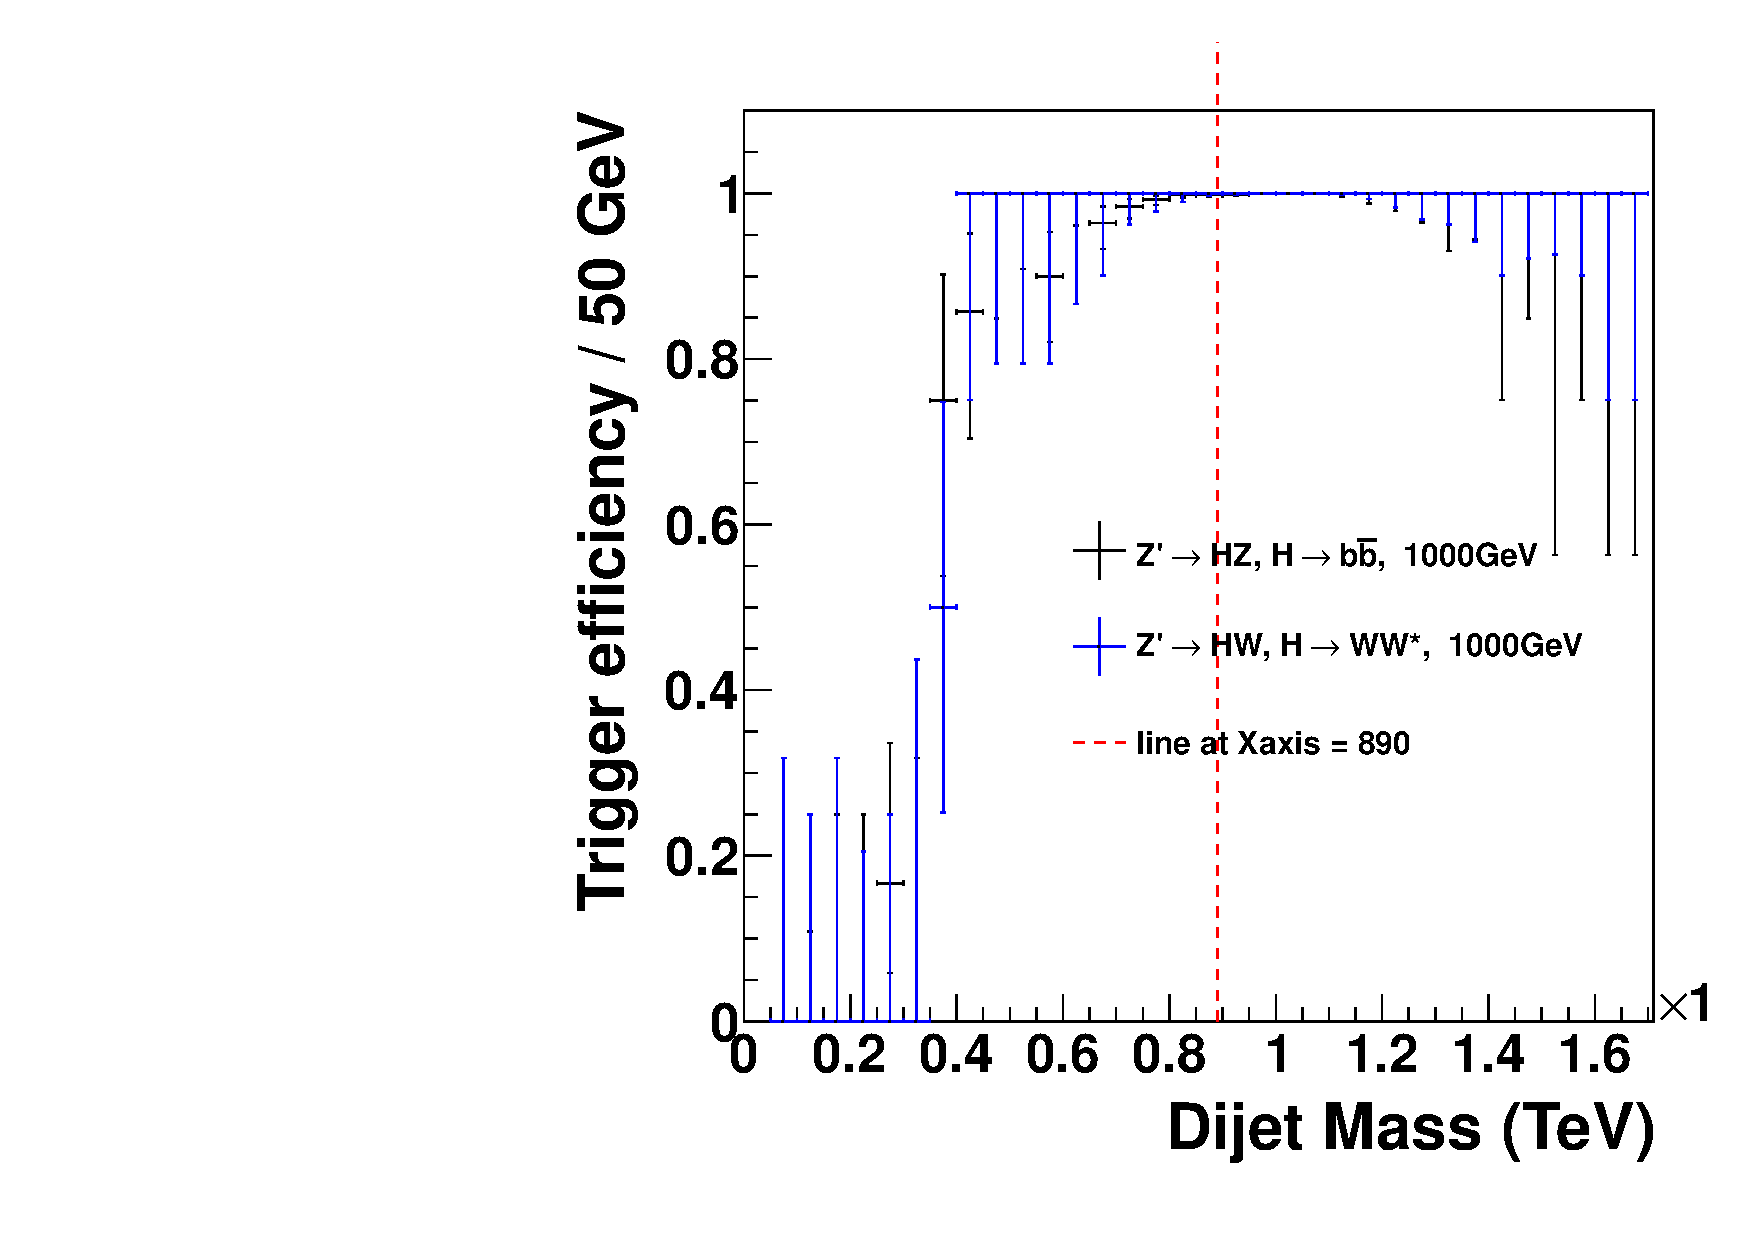
\includegraphics{EXO-14-009/figs/trigger-eff/TriggerStudySignal.pdf}} \\   
\caption[trigger efficiencies]{Reference trigger efficiency of signal MC.}
\label{fig:referencetrigger}
\end{figure}

\begin{figure}[htb]
\centering
     \resizebox{0.75\linewidth}{!}{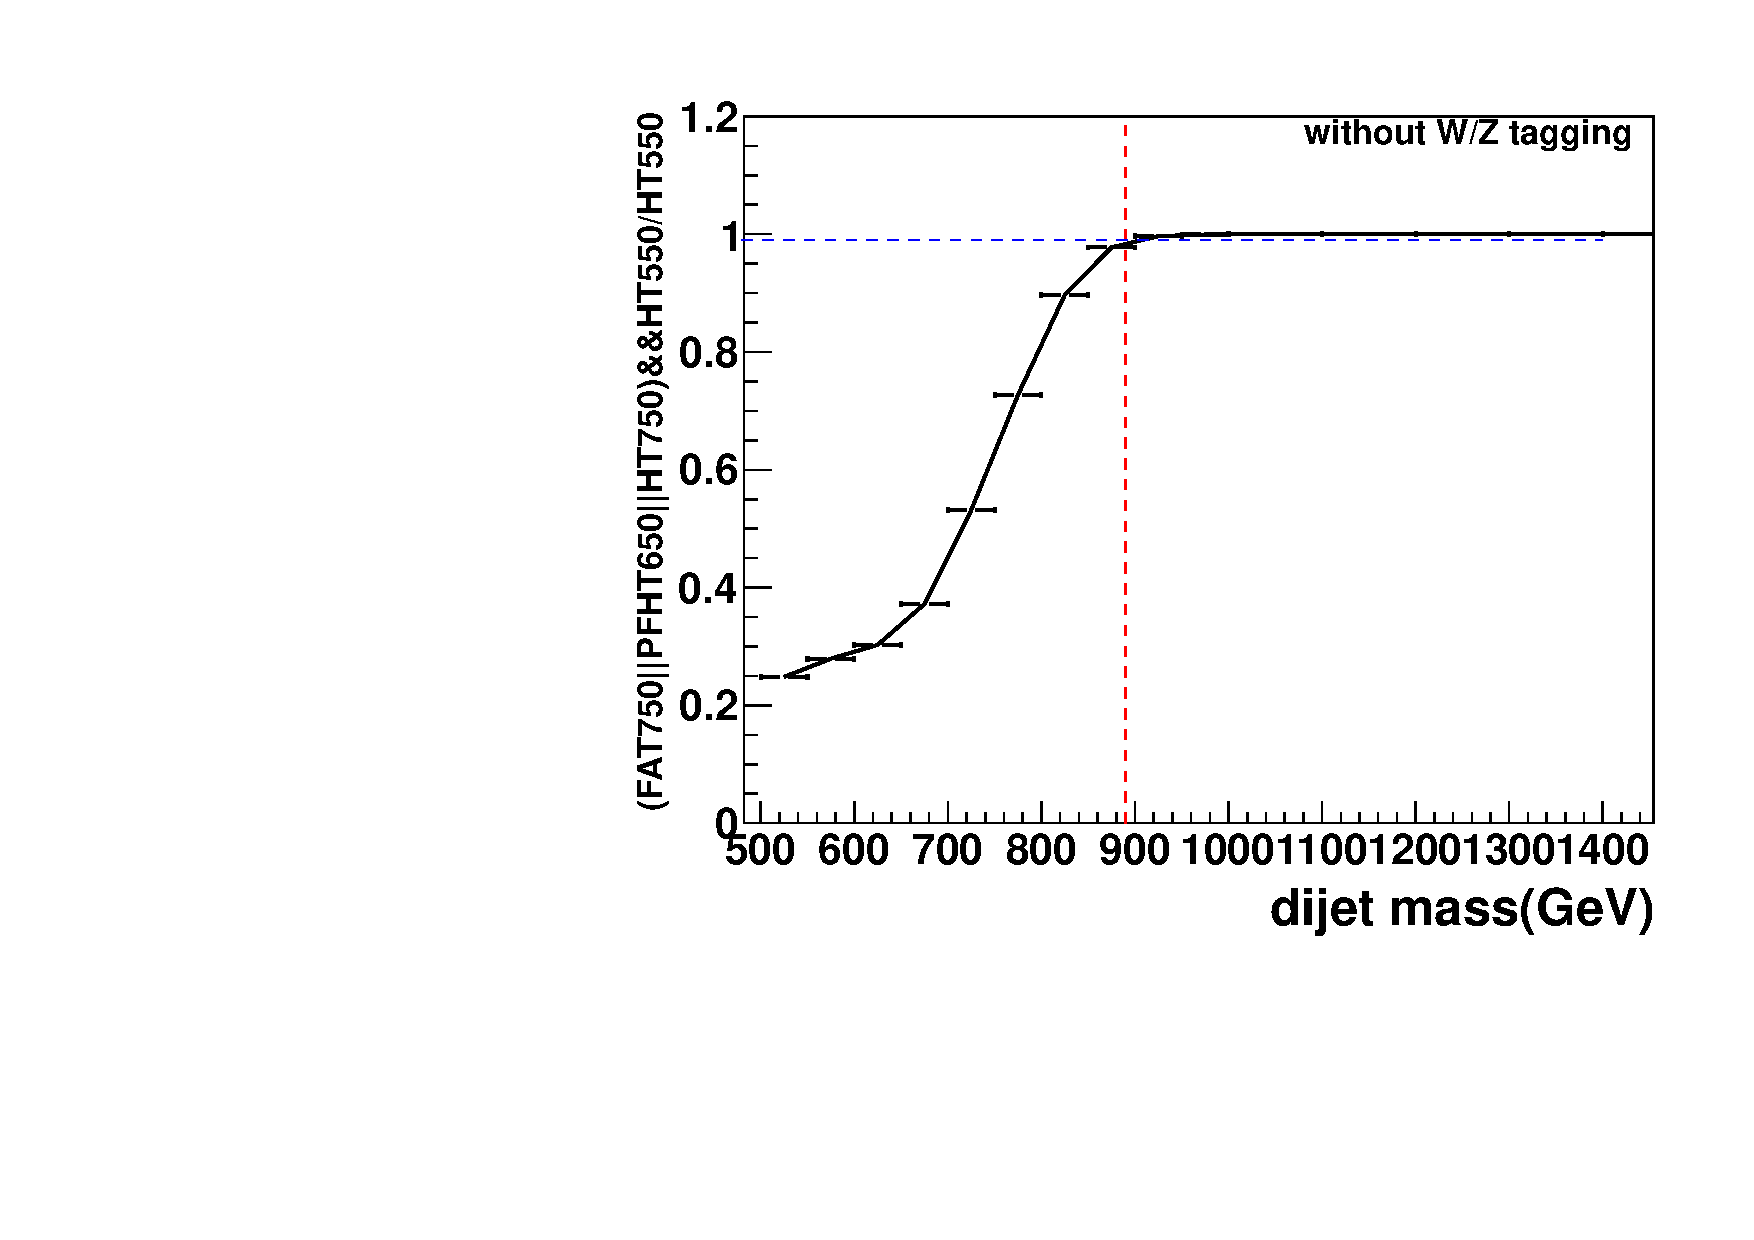
\includegraphics{EXO-14-009/figs/trigger-eff/Dataeff_withouttagging.pdf}} \\   
\caption[trigger efficiencies]{trigger efficiency for untagged data of fat\_750$\parallel$hlt\_pf(nopu)ht650$\parallel$hlt\_ht750 measured using data collected by lower threshold $h_t550$ trigger. the dashed red line is drawn at $m_{jj}$ equal 890 GeV, the blue line is at efficiency at 99$\%$. }
  \label{fig:trigger efficiencies part1}
\end{figure}

\begin{figure}[htb]
\centering
     \resizebox{0.75\linewidth}{!}{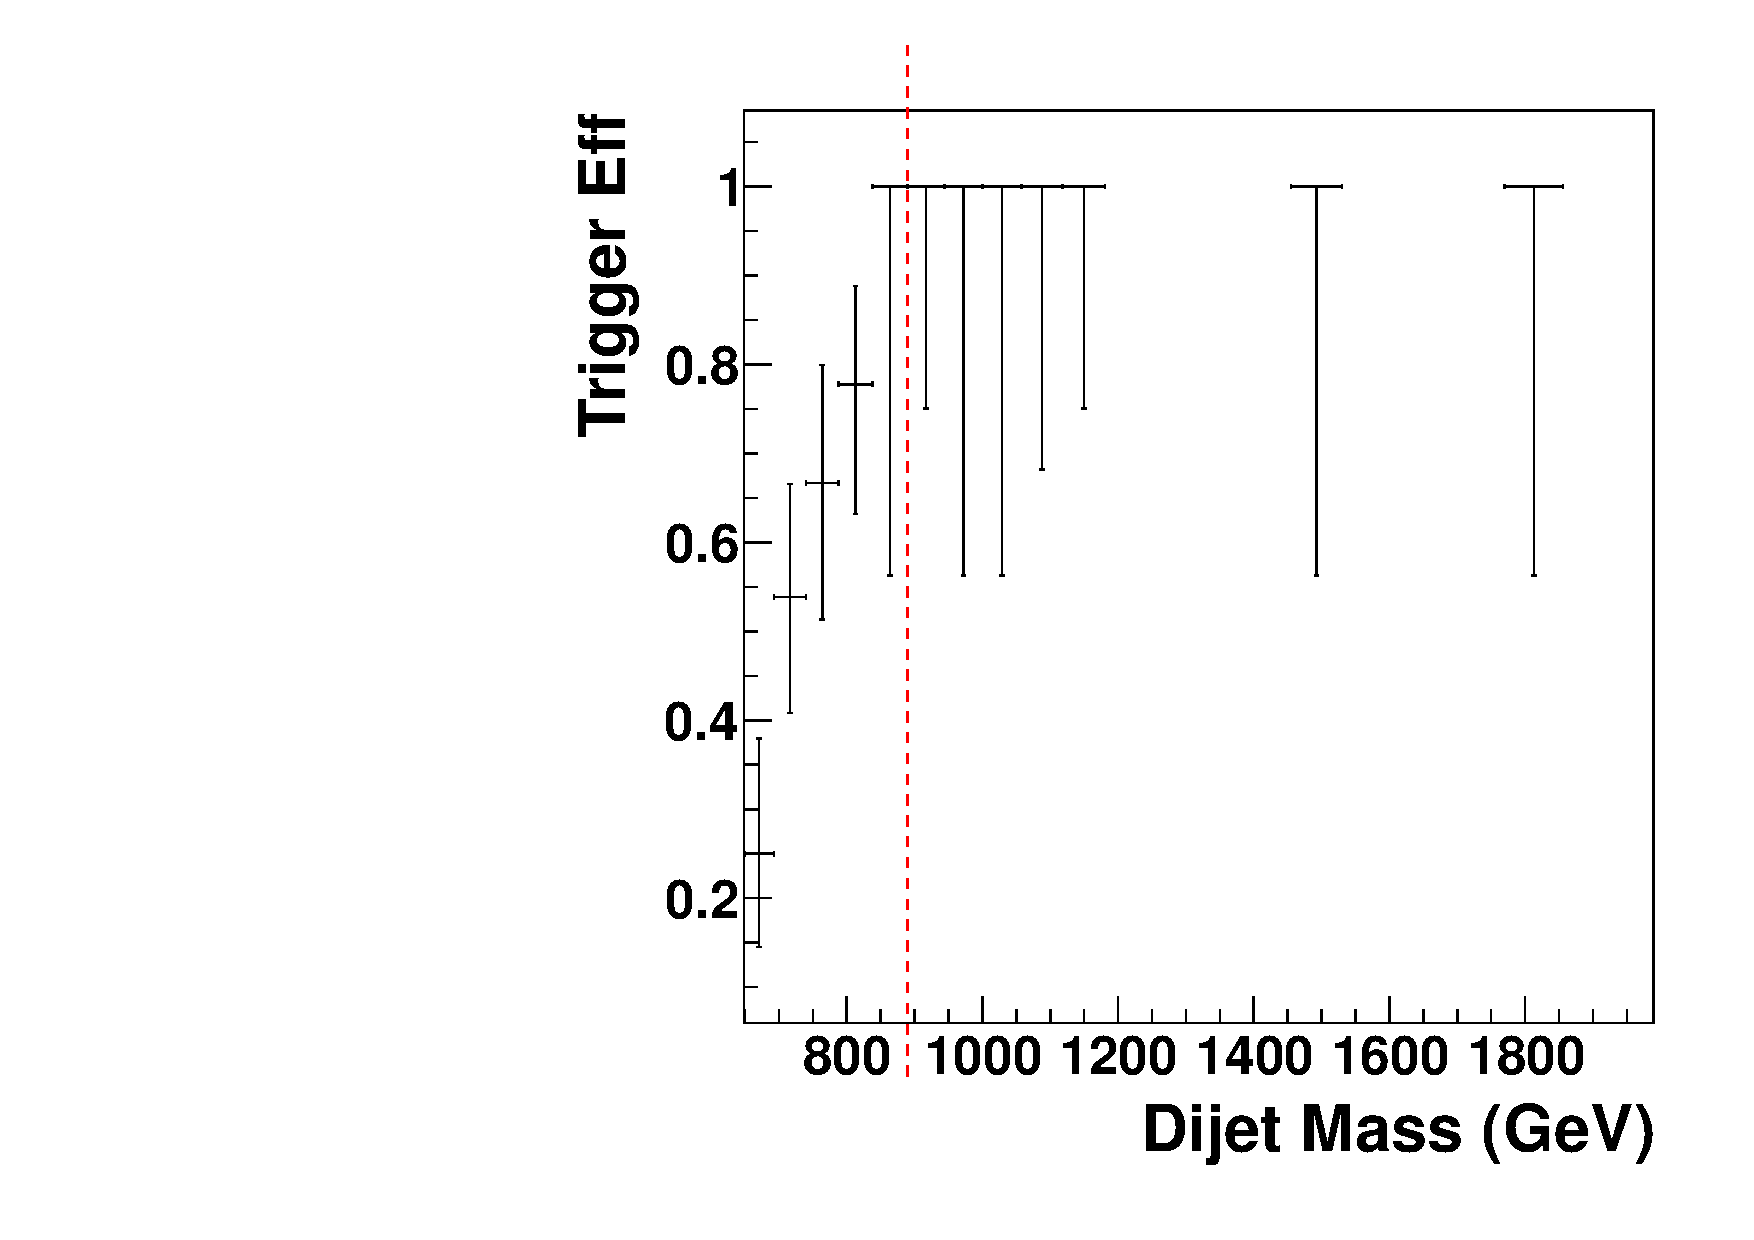
\includegraphics{EXO-14-009/figs/trigger-eff/DijetMassHbbPlotHighPurityBinned.pdf}}  \\
\caption[Trigger efficiencies]{Trigger efficiency for HbbVqq tagged data of FAT\_750$\parallel$HLT\_PF(NoPU)HT650$\parallel$HLT\_HT750 measured using data collected by lower threshold $H_T550$ trigger. The dashed red line is drawn at $m_{jj}$ equal 890 GeV. }
  \label{fig:trigger efficiencies part2}
\end{figure}

\begin{figure}[htb]
\centering
     \resizebox{0.75\linewidth}{!}{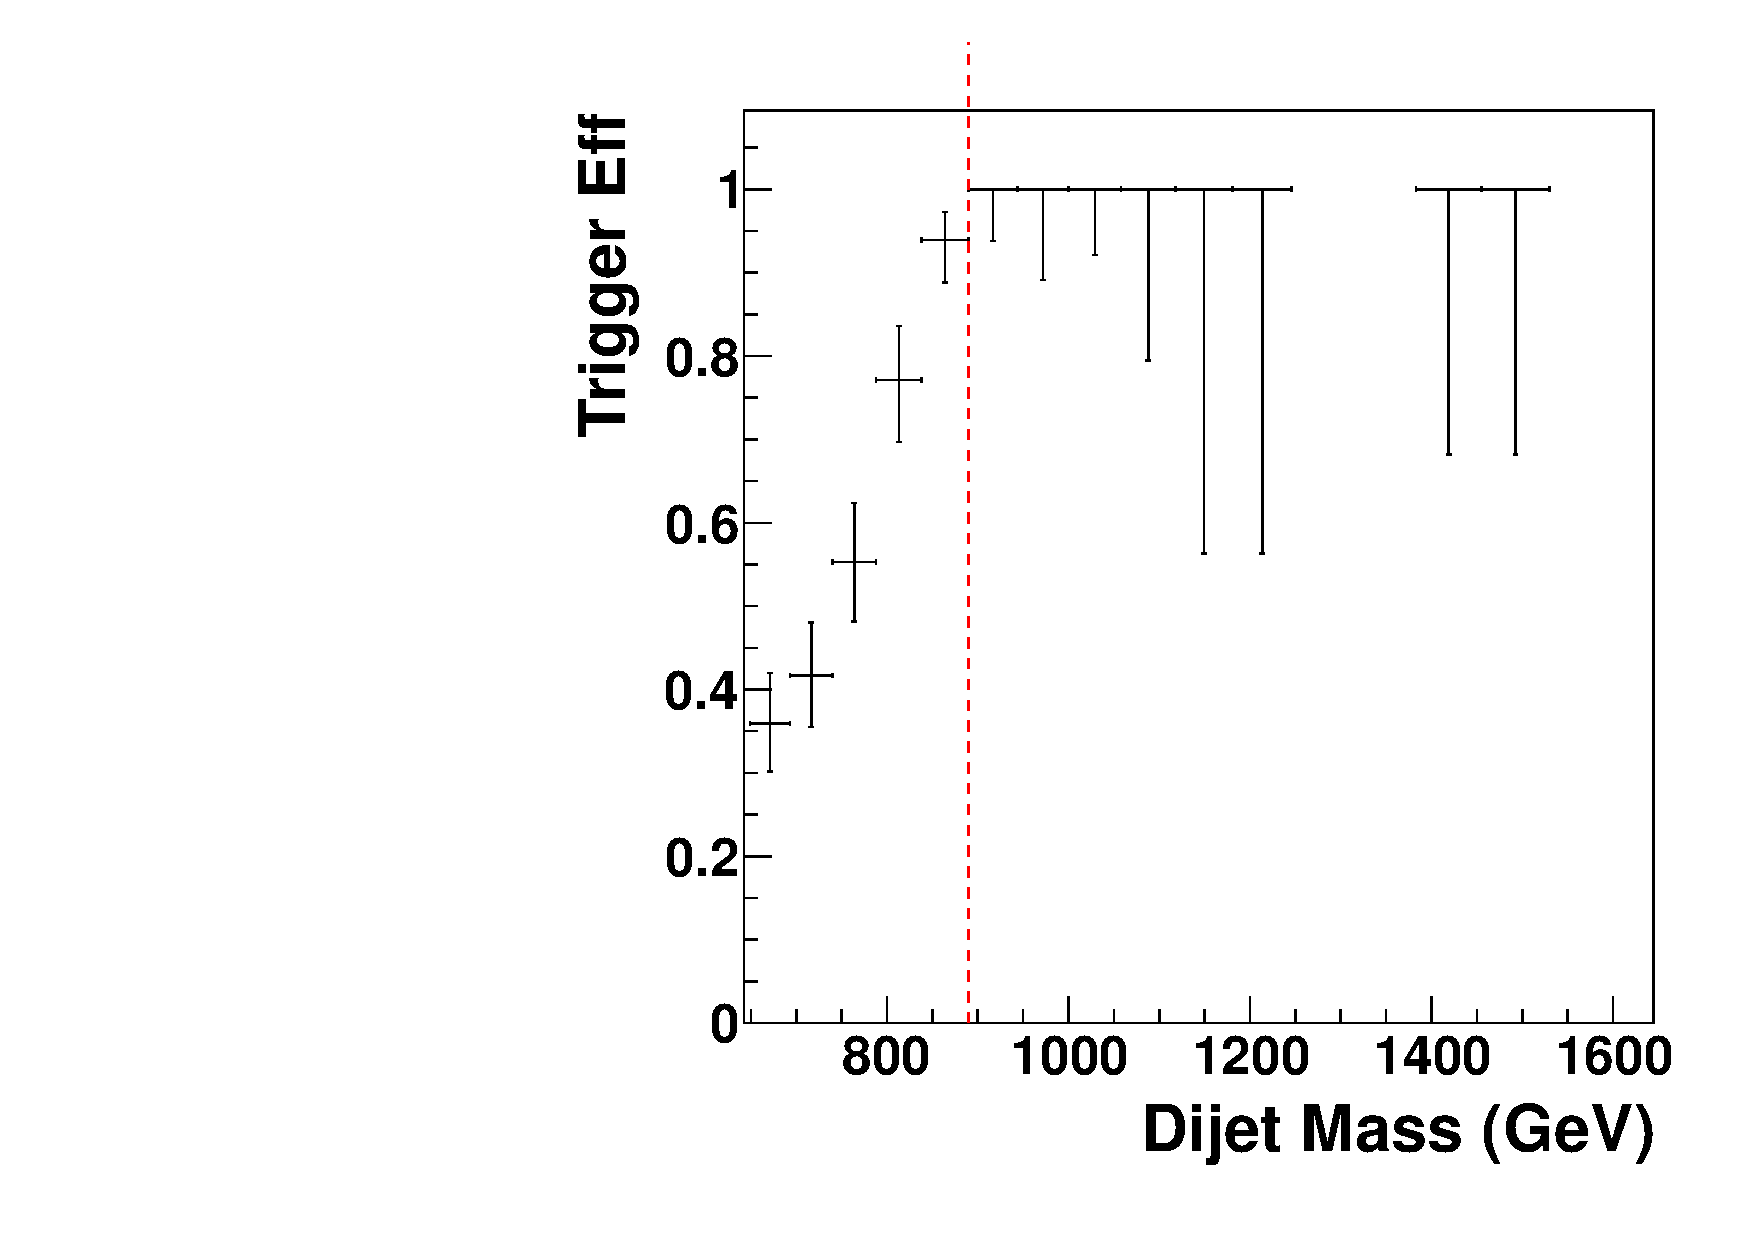
\includegraphics{EXO-14-009/figs/trigger-eff/DijetMassPlotBinnedHighP.pdf}} \\
\caption[Trigger efficiencies]{Trigger efficiency for HqqqqVqq tagged data of FAT\_750$\parallel$HLT\_PF(NoPU)HT650$\parallel$HLT\_HT750 measured using data collected by lower threshold $H_T550$ trigger. The dashed red line is drawn at $m_{jj}$ equal 890 GeV. }
  \label{fig:trigger efficiencies part3}
\end{figure}


\clearpage













